\subsection{Content Overview}

This report justifies how each of the components are designed in the Discussion section.
The algorithms behind the audio effects are based on the Infinite Impulse Response (IIR) algorithm \cite{SteveWinder2002C1},
due to lower computational cost and/or latency, as opposed to Finite Impulse Response (FIR).

Each audio effects and synthesizers are developed, and the perceptual audio
quality has already been evaluated. But signal analysis is conducted for audio effects only,
using some assessment tools, such as frequency response plots, waveforms from Audacity,
and impulse response plot.

\Cref{fig:main_daw_architecture} shows the diagram illustrating how the tracks should be arranged thread by thread. Each thread
holds a group of tracks mixed using a mini-mixer, which are then sent to the Master Mixer, and then to the PortAudio
callback engine. These threads run independently, not only to preserve callback times, but to prevent polling
or any scheduling conflicts from MIDI and Audio Inputs.

\begin{figure}[ht]
  \centering
  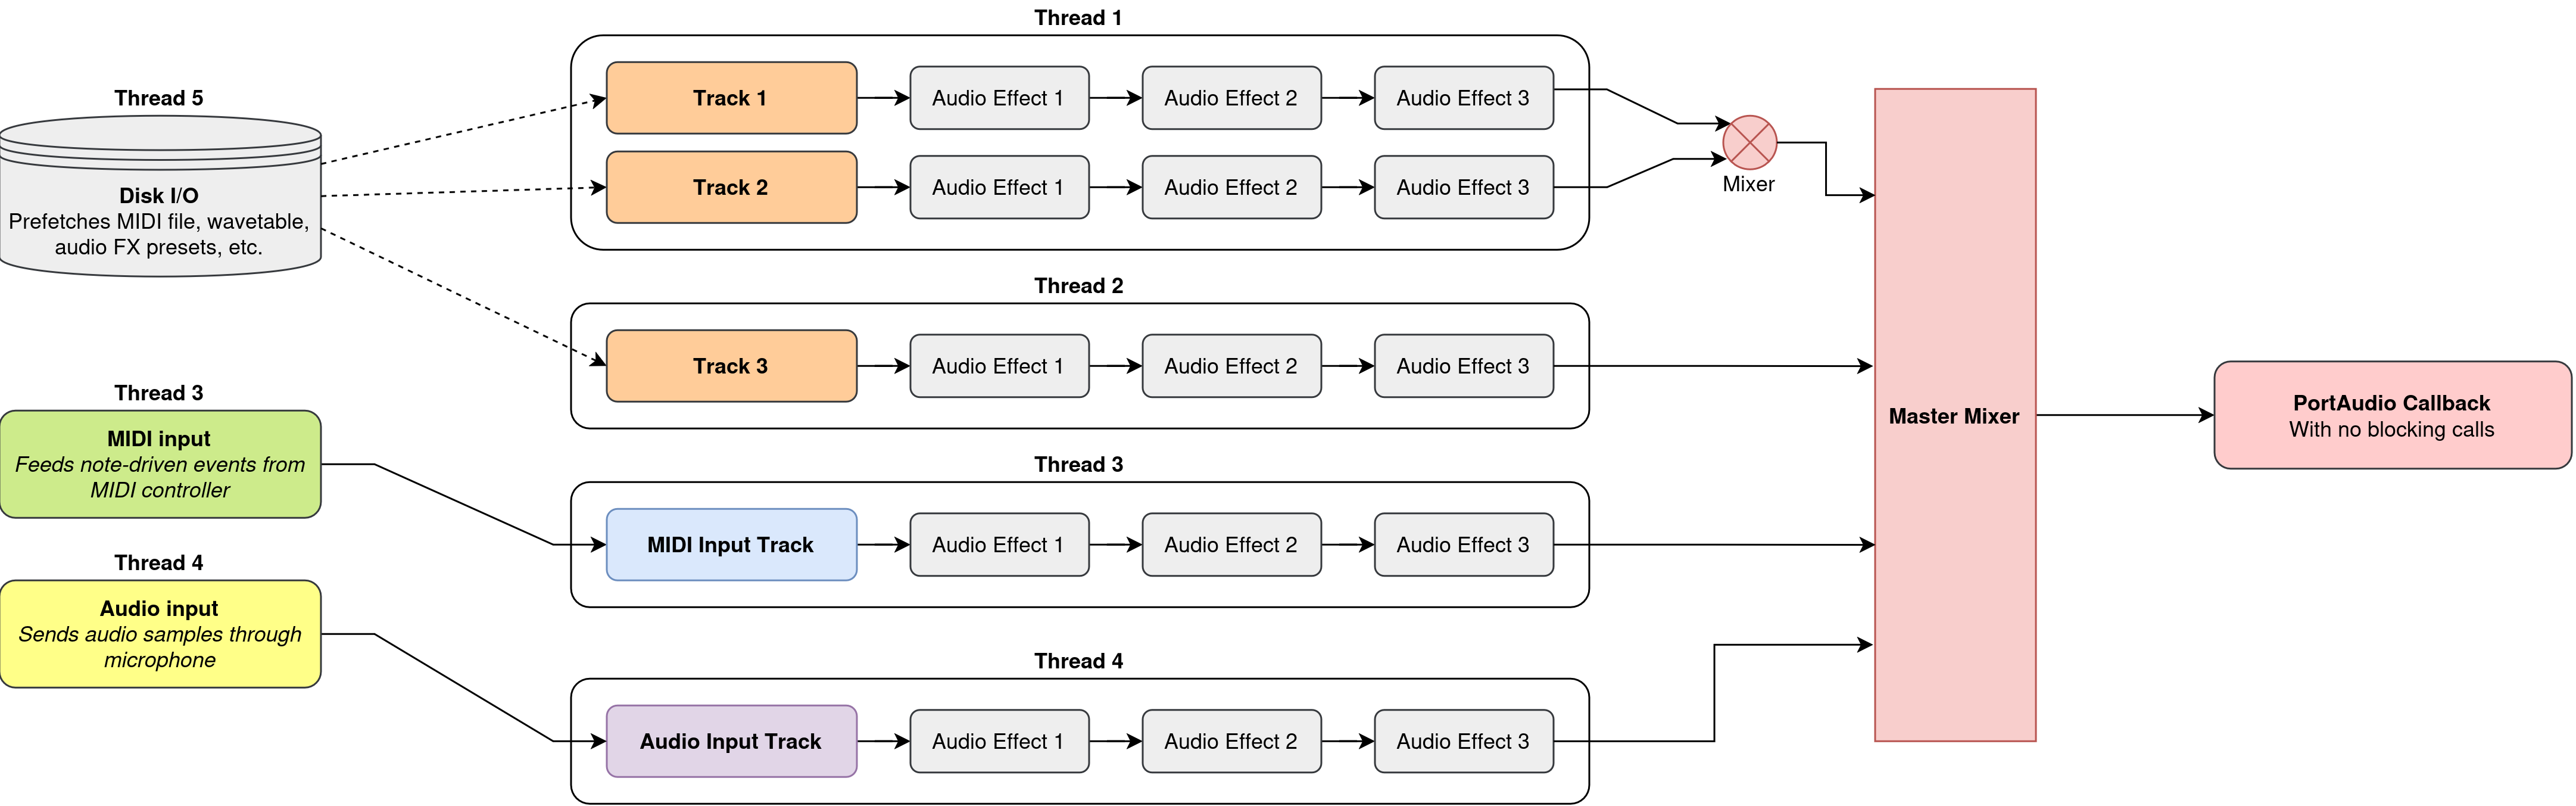
\includegraphics[width=\linewidth]{01_introduction/figures/architecture.png}
  \caption{Software Architecture of the DAW with Thread and Track Management}
  \label{fig:main_daw_architecture}
\end{figure}

Since the project is currently under construction, the actual 
stress test has not yet been performed due to limited number of components. But rather, an estimation
is conducted using a mockup DAW session containing only a list of instruments with no MIDI events,
and a look-up table containing measured execution times for each components. The Direct Acyclic Graph (DAG) 
technique \cite{susser_adc2025} is used to find the critical path, which is then used to calculate the overall 
execution time. This provides a reasonable amount of evidence to determine whether the tracks and audio effects 
would meet its deadline or not.